% Options for packages loaded elsewhere
\PassOptionsToPackage{unicode}{hyperref}
\PassOptionsToPackage{hyphens}{url}
%
\documentclass[
  12pt,
]{article}
\usepackage{lmodern}
\usepackage{amssymb,amsmath}
\usepackage{ifxetex,ifluatex}
\ifnum 0\ifxetex 1\fi\ifluatex 1\fi=0 % if pdftex
  \usepackage[T1]{fontenc}
  \usepackage[utf8]{inputenc}
  \usepackage{textcomp} % provide euro and other symbols
\else % if luatex or xetex
  \usepackage{unicode-math}
  \defaultfontfeatures{Scale=MatchLowercase}
  \defaultfontfeatures[\rmfamily]{Ligatures=TeX,Scale=1}
  \setmainfont[]{Times New Roman}
\fi
% Use upquote if available, for straight quotes in verbatim environments
\IfFileExists{upquote.sty}{\usepackage{upquote}}{}
\IfFileExists{microtype.sty}{% use microtype if available
  \usepackage[]{microtype}
  \UseMicrotypeSet[protrusion]{basicmath} % disable protrusion for tt fonts
}{}
\makeatletter
\@ifundefined{KOMAClassName}{% if non-KOMA class
  \IfFileExists{parskip.sty}{%
    \usepackage{parskip}
  }{% else
    \setlength{\parindent}{0pt}
    \setlength{\parskip}{6pt plus 2pt minus 1pt}}
}{% if KOMA class
  \KOMAoptions{parskip=half}}
\makeatother
\usepackage{xcolor}
\IfFileExists{xurl.sty}{\usepackage{xurl}}{} % add URL line breaks if available
\IfFileExists{bookmark.sty}{\usepackage{bookmark}}{\usepackage{hyperref}}
\hypersetup{
  pdftitle={Effects of a Defaunation Gradient on Tropical Forest Structure in Ivindo National Park, Gabon},
  pdfauthor={Tasha Griffiths, Israel Golden, Aubrey Knier, and Mishka Malinowski},
  hidelinks,
  pdfcreator={LaTeX via pandoc}}
\urlstyle{same} % disable monospaced font for URLs
\usepackage[margin=2.54cm]{geometry}
\usepackage{graphicx,grffile}
\makeatletter
\def\maxwidth{\ifdim\Gin@nat@width>\linewidth\linewidth\else\Gin@nat@width\fi}
\def\maxheight{\ifdim\Gin@nat@height>\textheight\textheight\else\Gin@nat@height\fi}
\makeatother
% Scale images if necessary, so that they will not overflow the page
% margins by default, and it is still possible to overwrite the defaults
% using explicit options in \includegraphics[width, height, ...]{}
\setkeys{Gin}{width=\maxwidth,height=\maxheight,keepaspectratio}
% Set default figure placement to htbp
\makeatletter
\def\fps@figure{htbp}
\makeatother
\setlength{\emergencystretch}{3em} % prevent overfull lines
\providecommand{\tightlist}{%
  \setlength{\itemsep}{0pt}\setlength{\parskip}{0pt}}
\setcounter{secnumdepth}{5}
\usepackage{booktabs}
\usepackage{longtable}
\usepackage{array}
\usepackage{multirow}
\usepackage{wrapfig}
\usepackage{float}
\usepackage{colortbl}
\usepackage{pdflscape}
\usepackage{tabu}
\usepackage{threeparttable}
\usepackage{threeparttablex}
\usepackage[normalem]{ulem}
\usepackage{makecell}
\usepackage{xcolor}

\title{Effects of a Defaunation Gradient on Tropical Forest Structure in Ivindo
National Park, Gabon}
\usepackage{etoolbox}
\makeatletter
\providecommand{\subtitle}[1]{% add subtitle to \maketitle
  \apptocmd{\@title}{\par {\large #1 \par}}{}{}
}
\makeatother
\subtitle{\url{https://github.com/israelgolden/GoldenGriffithsKnierMalinowski_ENV872_EDA_FinalProject}}
\author{Tasha Griffiths, Israel Golden, Aubrey Knier, and Mishka Malinowski}
\date{}

\begin{document}
\maketitle

\newpage
\tableofcontents 
\newpage
\listoftables 
\newpage
\listoffigures 
\newpage

\hypertarget{background-and-rationale}{%
\section{\texorpdfstring{\textbf{Background and
Rationale}}{Background and Rationale}}\label{background-and-rationale}}

Tropical forests throughout the world are experiencing changes in forest
structure and ecosystem services due to increasing hunting pressure,
resulting in plummeting animal populations\textsuperscript{1}. This
phenomenon, known as defaunation, has cascading effects throughout
ecosystems due to the disruption of intricate plant-animal interactions
that are responsible for shaping tropical forests\textsuperscript{1}.
Plant-animal interactions such as seed dispersal, seed predation,
seedling trampling, herbivory, and nutrient translocation are necessary
to shape forests. Through positive interactions such as the distribution
of seeds and nutrients and antagonistic interactions such as herbivory
and trampling - resulting in the opening up of the understory,
plant-animal interactions create opportunities for a variety of species
to succeed in the forest and increase plant diversity, richness, and
ecosystem services\textsuperscript{2}. For example,95\% of the trees in
the Afrotropical forests of LuiKotale in the Congo Basin depend on
animals for dispersal, demonstrating the necessity of plant-animal
interactions in these systems\textsuperscript{3}. The alteration or loss
of faunal communities in tropical forests has led to ``Empty Forest
Syndrome'', where a forest appears to be intact, but the animal
community is so depleted or non-existent that the forest no longer
functions as it did. These changes result in alterations to ecosystem
services, like carbon storage\textsuperscript{4}.

As defaunation continues to increase globally, there is little
understanding of the long-term effects of defaunation on tropical forest
diversity and ecosystem services. Tropical forests are responsible for
sequestering \textasciitilde40\% of the world's aboveground
carbon\textsuperscript{4}. Therefore, the impact of defaunation on
tropical forests may have detrimental effects for global carbon storage
and climate change projections. Further research is necessary to
understand the intricate interactions between defaunation, tropical
forests, and ecosystem services to illuminate these relationships and
advocate for policy changes and resource management. However, it is
essential to highlight that the underlying causes of defaunation are
top-down driven by the global economy, government regulations and
incentives, access to income and livelihoods,and ultimately quality of
life.

\hypertarget{study-overview-and-site}{%
\section{Study Overview and Site}\label{study-overview-and-site}}

Gabon, the second most forested country in the world, is located in
central western Africa and provides an ideal study site for
understanding the effects of defaunation on tropical forests (Figure 1).
The Afrotropical forests extending throughout Gabon are one of the last
strongholds for several endemic species including the forest elephant
\emph{(Loxodonta cyclotis)}. Ivindo National Park, one of 14 national
parks and presidential reserves, lies on the outskirts of several
villages and provides an excellent location to understand the
interactions of hunting pressure within tropical forests (Figure 2). A
study by Koerner et al.~in 2016 in this area described the existence of
a defaunation gradient radiating away from the villages and into Ivindo
national park. The results of the study showed that distance from
villages could be used as a proxy for defauntion and that every 10
kilometers traveled away from villages mammal richness would increase by
1.5 species\textsuperscript{5}.

In 2020 a project was started by the Poulsen Ecology Lab to establish
forest plots along the defaunation gradient to further explore the
relationship between forest structure and defaunation. As of 2022, 10
sites with a paired-plot design have been established (plots, n = 20).
Within the twenty 50 x 50m plots, all trees above 1.5 meters in height
have been tagged and measured. In six of these plots, tree species have
also been identified. Our analyses will focus on the complete data from
this subset of six plots(Figure 3). Makokou, the largest town in this
area also considered a regional capital, is indicated on the map to
demonstrate hunting pressure and indicate that the most defaunated plots
are those closest to Makokou while intact forests are farthest from
Makokou (Figure 3). Due to the scale of the map it appears there are
only 4 plots instead of 6, this is because of the paired - plot design
at the sites. Our dataset includes the paired plots DF 5A \& DF 5B and
DF 6A \& DF 6B. These pairs of plots are only separated by 100m,
therefore the points indicating the plots overlap on the below map
(Figure 3).

\begin{figure}
\centering
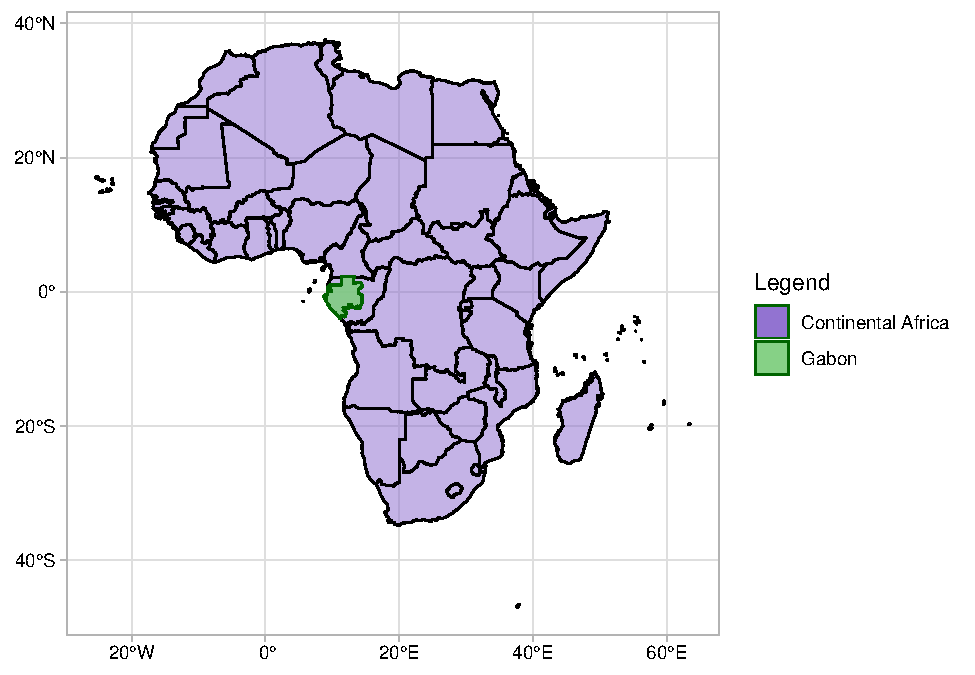
\includegraphics{GoldenGriffithsKnierMalinowski_ENV872_Project_files/figure-latex/Map of Gabon-1.pdf}
\caption{Map of Africa with Gabon Indicated}
\end{figure}

\begin{figure}
\centering
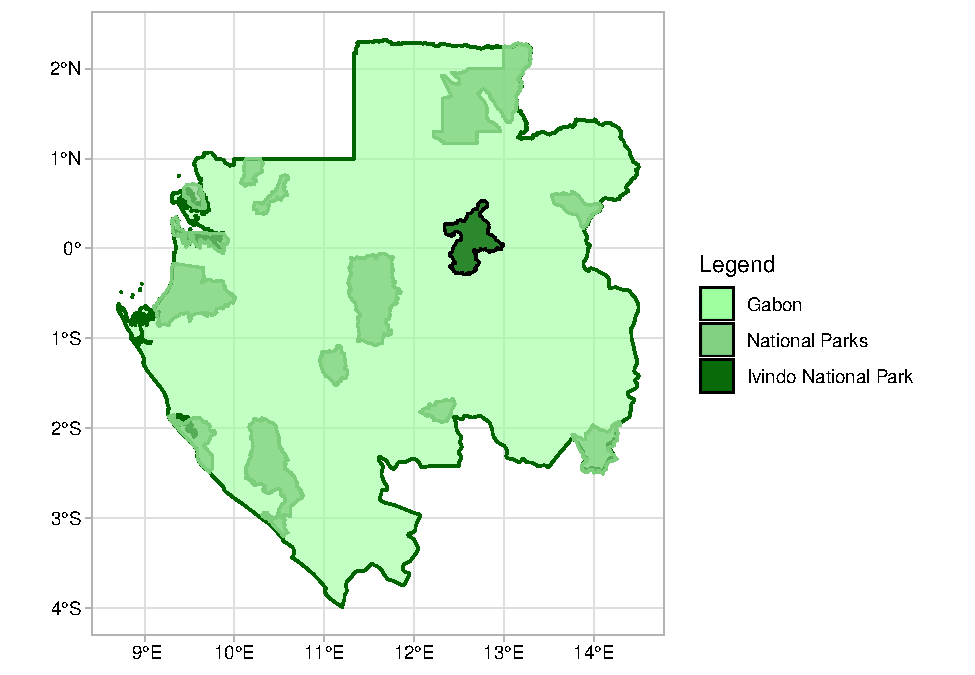
\includegraphics{GoldenGriffithsKnierMalinowski_ENV872_Project_files/figure-latex/Detailed Map of Gabon with parks-1.pdf}
\caption{Gabon's National Parks}
\end{figure}

\begin{figure}
\centering
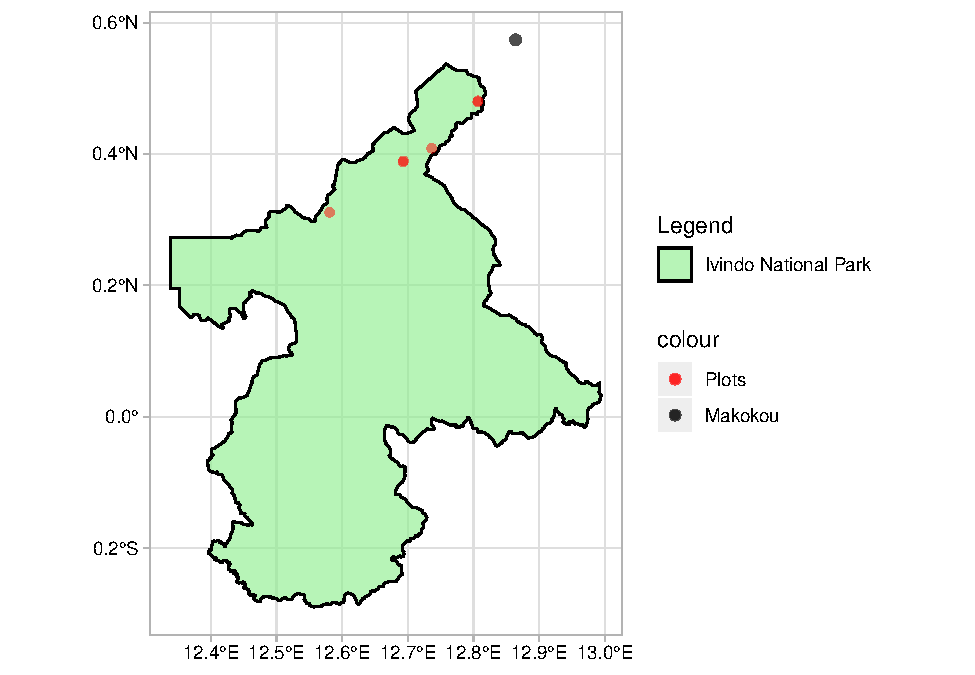
\includegraphics{GoldenGriffithsKnierMalinowski_ENV872_Project_files/figure-latex/Map of Ivindo with plots-1.pdf}
\caption{Forest Plots along a Defaunation Gradient in Ivindo National
Park, Gabon}
\end{figure}

\newpage

\hypertarget{research-questions}{%
\section{Research Questions}\label{research-questions}}

\textbf{Overarching Research Question:} How does defaunation affect
forest structure and composition in Ivindo National Park, Gabon?

\begin{itemize}
\tightlist
\item
  \emph{Research Question 1:} Does Diameter at Breast Height (DBH)
  change along a defaunation gradient?
\item
  \emph{Research Question 2:} Are there differences in Basal Area across
  a defaunation gradient?
\item
  \emph{Research Question 3:} Does species composition change along a
  defaunation gradient?
\end{itemize}

\newpage

\hypertarget{data}{%
\section{Data}\label{data}}

\hypertarget{dataset-information}{%
\subsection{Dataset Information}\label{dataset-information}}

This dataset is provided by the Pouslen Tropical Ecology Lab here at
Duke. A summary of the variables, variable descriptions, units, and
ranges are found in Table 1. The dimensions of the raw dataset are
below:

\begin{verbatim}
## [1] 45681    21
\end{verbatim}

\begin{table}[H]

\caption{\label{tab:unnamed-chunk-1}Raw Dataset Information}
\centering
\resizebox{\linewidth}{!}{
\begin{tabular}[t]{l|l|l|l}
\hline
Variable & Description & Unit & Range\\
\hline
E & Field expedition season & Season-Year & Winter - Summer 2021\\
\hline
Data\_entry & Name of individual inputting data to Excel & Name & \\
\hline
Date..dd.mm.yyyy. & Date of Excel data entry & Date/Month/Year & March 2021 - November 2022\\
\hline
File\_name & Photo file name of field data sheet & .JPG & \\
\hline
Date..dd.mm.yyyy..1 & Data of field data collection & Data of field data collection & June - January 2021\\
\hline
Note\_taker & Name of individual recording field data & Name & \\
\hline
Project & Defaunated forest (DF) or intact forest (IF) plot & Category & DF or IF\\
\hline
Plot & Unique plot identification & Category & 1-6 A-B\\
\hline
Grid & Within-plot grid where data were collected & Category & \\
\hline
TAG\_SUM & The most unique identifier, using plot grid and plant tag & Category & \\
\hline
Plant\_tag & Identifer assigned to each sample & Letter-Number Combination & \\
\hline
X\_coord & X coordinate of sample location & Degrees & 0.00 - 9.80\\
\hline
Y\_coord & Y coordinate of sample location & Degrees & 0.00 - 8.75\\
\hline
Tool & Tool used to measure diameter & Category & DBH or CP\\
\hline
POM & Point of measurement for diameter & Meters & 0.00 - 11.00\\
\hline
DBH.mm & Diameter at breast height (DBH) & Millimeters & 0.00 - 173.00\\
\hline
Height..meters. & Height of plant & Meters & 0.07 - 70.00\\
\hline
Type\_Field & Vegetation type or size class of plant & Category & Seedling, Sapling, Liana, Tree\\
\hline
Note\_Field & Miscellaneous field notes & Phrase & \\
\hline
ID & Latin species identification & Name & \\
\hline
Treatment & Future plot treatments (fungicide/insecticide) & Category & LMC, LME, MME, MMC\\
\hline
\end{tabular}}
\end{table}

\newpage

\hypertarget{data-cleaning}{%
\subsection{Data cleaning}\label{data-cleaning}}

With such a large dataset, data cleaning and wrangling was an essential
process for creating a manageable dataset that was relevant for
answering our research questions. First, we subset our selected six
plots for our analysis:

\begin{verbatim}
## [1] "DF_3B" "IF_2A" "DF_5A" "DF_5B" "DF_6A" "DF_6B"
\end{verbatim}

These plots were chosen out of the total 20 plots because they were the
only ones that had species identifications attached to samples, which
was needed for our investigation of how defaunation affects species
composition.

Next, we only selected columns that contained variables of interest:

\begin{verbatim}
## [1] "Project.Plot" "Plant_tag"    "DBH_mm"       "Height_m"     "Veg_Type"    
## [6] "ID"
\end{verbatim}

We removed absent or unreasonable values from the dataset. This involved
simply removing blank cells or ``NAs'', as well as measurements that
were likely incorrect, probably as a result of improper unit
conversions. Additionally, we improved uniformity in the dataset by
removing samples that had a height less than 1.5m and lianas. This was
because not all plots measured individuals smaller than 1.5m, and height
measurements for lianas are less reliable, so we decided to only analyze
trees. We also found some instances in our data where samples were
relatively tall yet had a very small DBH. Since this likely due to a
data collection or entry error, we removed any samples that had a DBH
less than 1mm and a height above 1.5m to improve accuracy.

We also added in variables to support our research questions and
analyses. We created two new columns: ``Status'' referring to defaunated
or intact study plots and ``Distance\_km'' from Makokou (Table 2). The
categorical variable, ``Status'', will help with data visualization, and
the ``Distance\_km'' variable will be used as a proxy from the
defaunation gradient in our analyses. A sample of our cleaned dataset is
shown in Table 3.

\begin{table}[H]

\caption{\label{tab:unnamed-chunk-4}Added Variables to Dataset}
\centering
\resizebox{\linewidth}{!}{
\begin{tabular}[t]{l|l|l|l}
\hline
Variable & Description & Unit & Range\\
\hline
Status & Indicates whether each plot is defaunated or intact forest & Category & Defaunated - Intact\\
\hline
Distance\_km & Distance of each plot from Mokokou & Kilometers & 8.177 - 40.224\\
\hline
\end{tabular}}
\end{table}

\begin{table}[H]

\caption{\label{tab:head/columns}Head of Cleaned Dataset}
\centering
\resizebox{\linewidth}{!}{
\begin{tabular}[t]{l|l|r|r|l|l|l|r}
\hline
Project.Plot & Plant\_tag & DBH\_mm & Height\_m & Veg\_Type & ID & Status & Distance\_km\\
\hline
DF\_3B & 1554 & 558.8 & 30.0 & Tree & Heisteria parvifolia & Defaunated & 20.195\\
\hline
DF\_3B & 69 & 15.8 & 2.4 & Tree & Dialium pachyphyllum & Defaunated & 20.195\\
\hline
DF\_3B & 4371 & 11.7 & 1.8 & Sapling & Scorodophloeus zenkeri & Defaunated & 20.195\\
\hline
DF\_3B & 607 & 19.4 & 2.5 & Tree & Odjendja gabonensis & Defaunated & 20.195\\
\hline
DF\_3B & 7150 & 21.5 & 3.7 & Tree & Scorodophloeus zenkeri & Defaunated & 20.195\\
\hline
DF\_3B & 7110 & 65.0 & 7.5 & Tree & Centroplacus glaucinus & Defaunated & 20.195\\
\hline
\end{tabular}}
\end{table}

Accidental misspellings are common in datasets such as this with
thousands of manual entries of complex Latin species names. This is a
concern because two samples that are supposed to be the same species,
but have different spellings, will not be identified as the same species
in our analyses. By looking at a list of the unique species names in the
dataset, we found this to be the case in several instances. Identifying
these errors and correcting them was quite labor intensive and can only
be completed with the human eye and personal judgment as to what names
are meant to be the same. Before cleaning the species names, there were
349 ``species''; after correcting for spelling mistakes, there were only
323 species. This means that 26 ``species'' were falsely identified
prior to data cleaning.

The dimensions of the processed, clean dataset are as follows:

\begin{verbatim}
## [1] 6279    8
\end{verbatim}

\newpage

\hypertarget{methods}{%
\section{Methods}\label{methods}}

\hypertarget{research-question-1}{%
\subsection{Research Question 1}\label{research-question-1}}

\emph{Does Diameter at Breast Height (DBH) change along a defaunation
gradient?}

We began by analyzing our data through an examination of how DBH
distribution (size classes) changes along the defaunation gradient.
Diameter at Breast Height (DBH) is a measurement of the circumference of
a tree trunk 1.37 meters or 4.5 feet above the ground. DBH may be used
to understand the effect of defaunation within a stand. For example, a
high frequency of thinner trees would indicate an earlier successional
pattern and a higher frequency of larger/wider trees a more mature stand
with less disturbance. DBH was taken in millimeters for all trees above
1.5m in height within the plots. We used a ggplot visualization and
histogram in order to understand the frequency and size distribution of
DBH of individual trees within each of the six plot sites. We added all
sites with a facet wrap in order to directly compare distribution with
the same scale. The x-axis is DBH in mm, with default bin sizes and the
y-axis is frequency of occurrence. The sites were also ordered in
distance from Makokou with sites EF\_5A and EF\_5B being the closest and
IF\_2A being the farthest away.

\hypertarget{research-question-2}{%
\subsection{Research Question 2}\label{research-question-2}}

\emph{Are there differences in Basal Area across a defaunation
gradient?}

Next, we used the cleaned data to generate summaries of stand
characteristics at the plot level. These characteristics included the
total basal area of each site, the standard deviation of basal area
among individual trees, the species richness of each site, and the basal
area per hectare of each plot. Basal area is the cross-sectional area of
a tree at breast height. By summing basal area for a plot, the result
provides a means of understanding the tree density of a stand. Basal
area has implications for forest health, competition, and growth
dynamics. Basal area was calculated by mutating the DBH column to
reflect the basal area of each observation. DBH can be converted to
basal area - in terms of square cm - from mm with the formula BA =
((pi*d\textsuperscript{2})/4)/100. The basal area for each site was then
summed and converted to square meters for visualization. These summary
values allowed for comparison of forest structure and species richness
between project plots.

\hypertarget{research-question-3}{%
\subsection{Research Question 3}\label{research-question-3}}

\emph{Does species composition change along a defaunation gradient?}

We then calculated and visualized the proportion of basal area that each
genera contributed to overall basal area for each plot. Unique species
were too numerous for effective visualization so we used unique genera
to provide a visual representation of the diversity of tree lineages at
each plot. This was accomplished by extracting the first word (i.e., the
genus) from the species ID column to create a genus column. The basal
area for each genus at each plot was then summed and visualized
alongside the basal area of other genera to show the overall
contribution of each genus to the plot's basal area.

\hypertarget{research-question-synthesis}{%
\subsection{Research Question
Synthesis}\label{research-question-synthesis}}

Finally, we sought to uncover a relationship between distance from
Makokou and forest structure and species richness with a linear model.
The model describes basal area per hectare as a function of distance
from Makokou and total number of unique species for each plot. Distance
from Makokou serves as a proxy for position along the defaunation
gradient where shorter distances are assumed to be more defaunated and
farther distances are considered to be intact, faunated forest. The null
hypothesis of both of these models is that there is no relationship
between distance from Makokou (i.e., position along the defaunation
gradient). Alternatively, if an explanatory variable in the model is
deemed significant, it could provide some insight into how the
defaunation gradient affects either basal area or species richness.

\hypertarget{results}{%
\section{Results}\label{results}}

\hypertarget{research-question-1-1}{%
\subsection{Research Question 1}\label{research-question-1-1}}

\emph{Does Diameter at Breast Height (DBH) change along a defaunation
gradient?}

The below visualizations indicate that all sites have a much higher
frequency of thinner trees - smaller than 150mm in DBH (Figures 4 \& 5).
However, upon adjusting the x-axis scale, it is easier to see a full
histogram of the plots. These visualizations led to two key findings:

\begin{enumerate}
\def\labelenumi{\arabic{enumi}.}
\item
  Plots closer to the city have higher overall frequencies and higher
  frequencies of large DBH trees. For example, plots DF\_5A and DF\_5B
  have higher frequencies of larger trees.
\item
  Plots farther away from the city, such as IF\_2A has fewer overall
  trees and the trees that are present are much thinner in DBH.
\end{enumerate}

Since DBH for all of the plots was skewed to the smaller size class,
this tends to indicate more defaunation in all plots. Also it was
unexpected to have larger DBH trees closer to town and thinner trees in
the single `intact' forest plot. One would expect the opposite to be
true with more defaunation close to the town and wider trees farthest
away. One potential explanation for this may be the existence of
remaining old growth trees in these plots due to the short time scale
for defaunation in this area (approximately the last 50 years). Over a
greater time period the large trees would senesce and die and not be
replaced due to lack of seed dispersers.

\begin{figure}
\centering
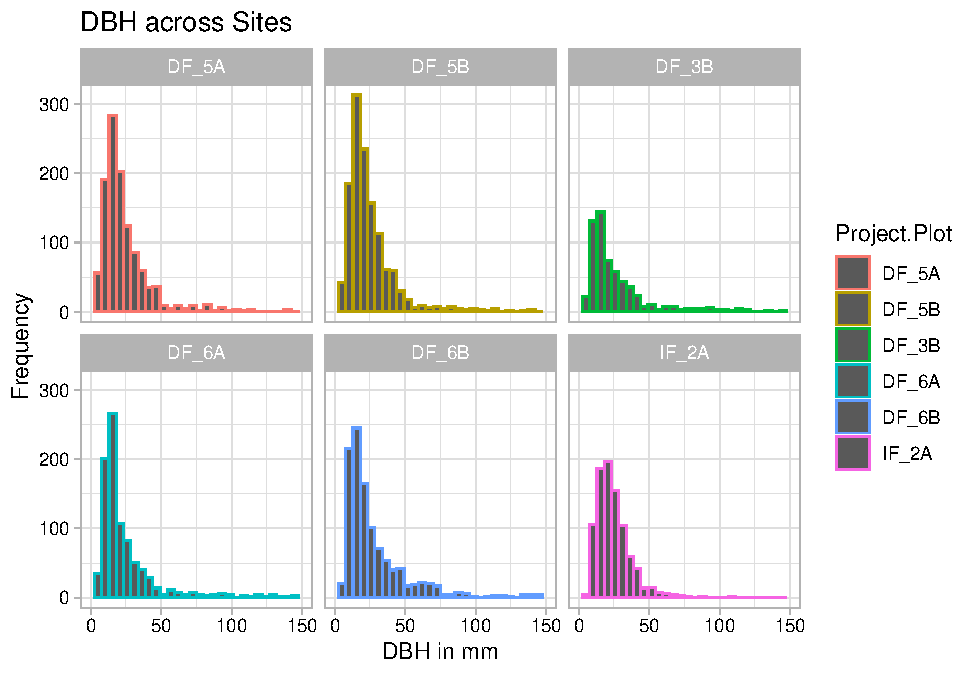
\includegraphics{GoldenGriffithsKnierMalinowski_ENV872_Project_files/figure-latex/unnamed-chunk-5-1.pdf}
\caption{Distribution of DBH Size Classes per Plot}
\end{figure}

\begin{figure}
\centering
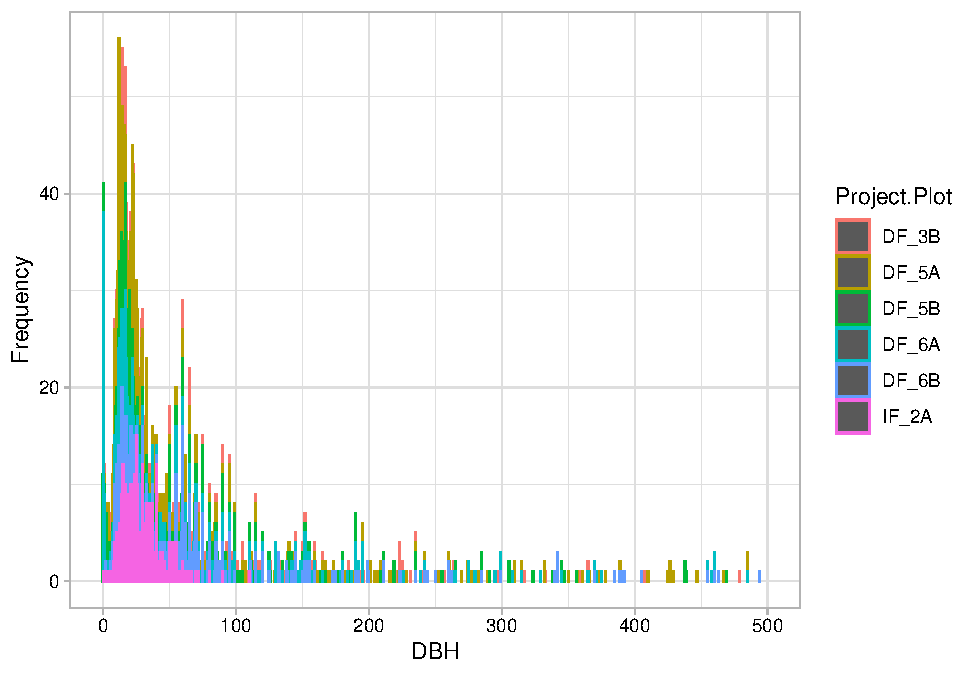
\includegraphics{GoldenGriffithsKnierMalinowski_ENV872_Project_files/figure-latex/unnamed-chunk-7-1.pdf}
\caption{Distribution of DBH Size Classes Across Plots}
\end{figure}

\hypertarget{research-question-2-1}{%
\subsection{Research Question 2}\label{research-question-2-1}}

\emph{Are there differences in Basal Area across a defaunation
gradient?}

Results of this exploratory analysis reveal differences in basal area
and species richness for each plot. As basal area is a function of DBH,
the distribution of basal area across plots mirrored that of its DBH
distribution (Figure 4). This result affirms that trees at each site are
mostly small with few trees above 10 cm2 of basal area and even fewer -
if any - above 20 cm\textsuperscript{2}. Species richness values ranged
between 79 and 148; but four out of the six plots had a mean species
richness of 85 (Figure 6). The two plots with the greatest species
richness were DF\_6A and DF\_6B which had 141 and 148 unique species
respectively. Total basal area at each plot ranged from 0.92
m\textsuperscript{2} to 15.35 m\textsuperscript{2}. The plots with the
greatest basal area were plots DF\_5A and DF\_6B which had
15.35m\textsuperscript{2} and 11.66 m\textsuperscript{2} respectively.
Interestingly, the intact forest plot , IF\_2A, had the lowest basal
area at 0.92 m\textsuperscript{2}. Given IF\_2A's high species richness
but low basal area, these results seem to suggest that IF\_2A has many
small trees, but few large ones. Overall, there does not appear to be a
strong relationship between number of tree species and basal area.

\begin{figure}
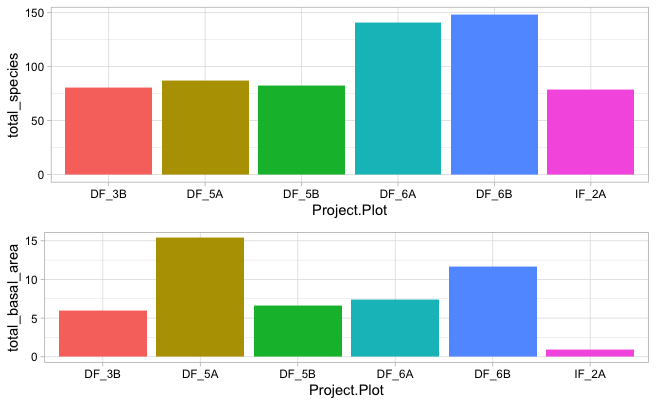
\includegraphics[width=0.95\linewidth]{./GoldenGriffithsKnierMalinowski_ENV872_Project_files/figure6} \caption{Species Richness and Basal Area by Plot}\label{fig:unnamed-chunk-9}
\end{figure}

\hypertarget{research-question-3-1}{%
\subsection{Research Question 3}\label{research-question-3-1}}

\emph{Does species composition change along a defaunation gradient?}

By combining genus richness with basal area into treeplots, we are able
to compare the abundance of tree genera at each plot. Specifically,
treeplots allow us to visually represent the contribution of basal area
by each genus at each plot. No single tree genera was overwhelmingly
dominant across all plots. Rather, each plot had one to three genera
that contributed a plurality of the basal area. Plot DF\_6A, which had
the greatest number of unique species, was dominated by Beilschmiedia
(14\% of basal area or 10,438 cm\textsuperscript{2}), Petersianthus (9\%
of basal area or 6,268 cm\textsuperscript{2}), and Celtis (8.5\% of
basal area or 5,986 cm\textsuperscript{2}) species (Figure 7).
Meanwhile, IF\_2A, which had the smallest amount of basal area, was
dominated by a single genus: Thomandersia (56\% of basal area or 5202
cm\textsuperscript{2}) (Figure 8). Overall, species composition did
change along the defaunation gradient, but there were no predictable or
observable trends that dictated these changes.

\begin{figure}
\centering
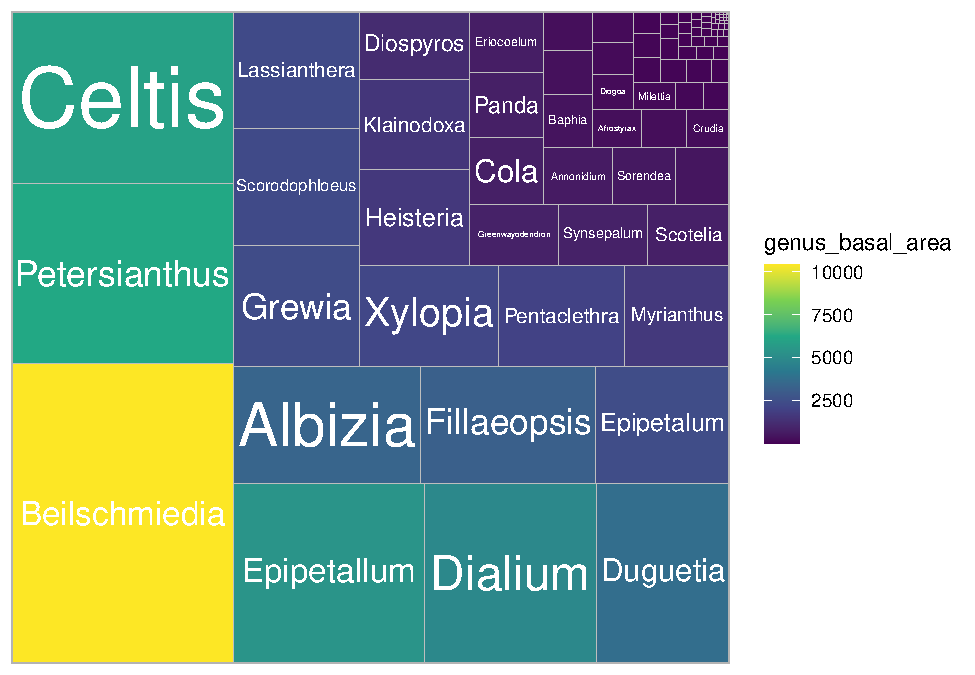
\includegraphics{GoldenGriffithsKnierMalinowski_ENV872_Project_files/figure-latex/unnamed-chunk-10-1.pdf}
\caption{DF\_6A Tree Plot}
\end{figure}

\begin{figure}
\centering
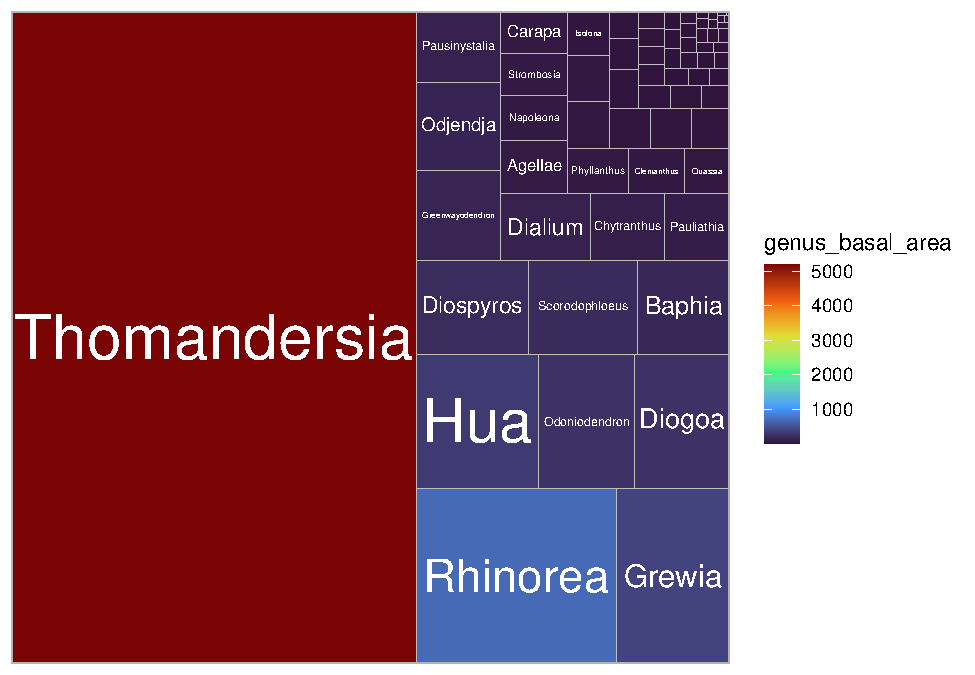
\includegraphics{GoldenGriffithsKnierMalinowski_ENV872_Project_files/figure-latex/unnamed-chunk-11-1.pdf}
\caption{IF\_2A Tree Plot}
\end{figure}

\newpage

\hypertarget{research-question-synthesis-1}{%
\subsection{Research Question
Synthesis}\label{research-question-synthesis-1}}

Finally, based on the data from these plots there does not appear to be
a meaningful relationship between distance from Makokou, species
richness and basal area. Based on our correlation plot, basal area at
each plot appears to be negatively correlated with distance from
Makokou. However, when we modeled the relationship basal area as
explained by distance from Makokou and species richness the result was
not significant (p = 0.16). As such, we cannot reject the null
hypothesis that there is no relationship between distance from Makokou
and basal area. The relationship between distance from Makokou and basal
area had a p-value of 0.11. Though this is not significant, it does
suggest that there is a negative correlation between these two values
and that with each additional kilometer from Makokou, basal area is
reduced by 1.3 m\textsuperscript{2} (Figure 9).

\begin{figure}
\centering
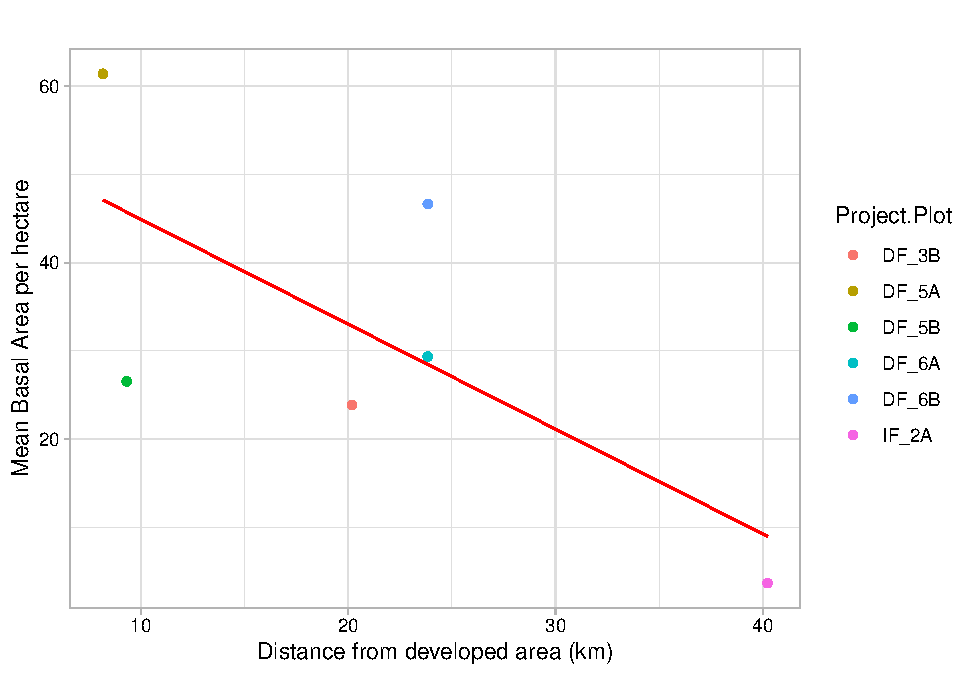
\includegraphics{GoldenGriffithsKnierMalinowski_ENV872_Project_files/figure-latex/fig 9-1.pdf}
\caption{Basal Area and Distance to Developed Area}
\end{figure}

\newpage

\hypertarget{summary-and-conclusions}{%
\section{Summary and Conclusions}\label{summary-and-conclusions}}

\begin{figure}
\centering
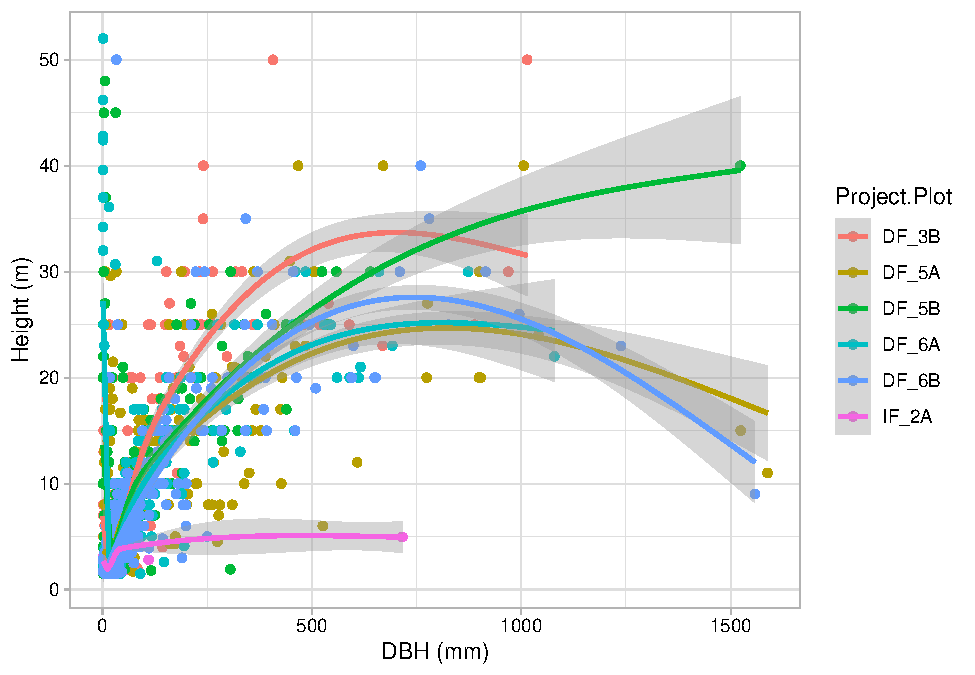
\includegraphics{GoldenGriffithsKnierMalinowski_ENV872_Project_files/figure-latex/plot of DBH vs height-1.pdf}
\caption{Height vs.~DBH Comparison}
\end{figure}

Figure 10 shows that there are clearly errors in the data. The
relationship between height and DBH should follow a positive linear
trend especially in early life stages for a tree through seedling,
sapling, juvenile, and early adult life stages. As trees mature they may
slow their growth and reach an asymptote or threshold for their height,
but may continue to increase in diameter slowly. This trend is not shown
for a large portion of the data. Of particular concern is the large
spread of heights at small DBH values. It is unrealistic to believe that
a 40m tree may have a DBH as small as 10mm. Therefore, it is likely that
there is a high level of error within the dataset. This error may have
occurred in 3 places. First, during data collection in the field, the
measurement may have been taken incorrectly. Secondly, the data may have
been recorded incorrectly in the field or lastly when data was
transferred from the paper data collection sheets into excel it may have
been entered incorrectly. This is likely an issue of unit conversion and
will ideally be resolved by checking the dataset against the raw data
sheets. However, this peculiar relationship between height and DBH
likely impacted the results of this analysis and may explain why many of
the results do not agree with expected outcomes.

However, our data cleaning and analyses have provided an essential
starting point to further explore the effects of defaunation on tropical
forest structure and composition within Ivindo National Park, Gabon.
Although the results differ from our expected outcomes a key finding in
this exploration has been uncovering errors in the dataset that may lead
to faulty results or ecologically uninterpretable findings. We were able
to address our \emph{overarching research question} - ``How does
defaunation affect forest structure and composition in Ivindo National
Park, Gabon?'' - although further data collection, data cleaning, and
analysis is necessary. Overall, no specific trends were found between
defaunation (using distance to village as a proxy for defaunation) and
our forest structure and composition variables (DBH, basal area, and
genus richness). In addition to the discrepancies in the DBH and height
data (Figure 10) another factor contributing to lack of significant
results may be that amongst the 6 plots used in our analyses only one
was considered intact forest. A greater dataset including the remaining
plots along the gradient may help to draw more conclusions about these
relationships and uncover any trends. Currently a team of Gabonese
researchers and colleagues from the Poulsen Lab are conducting this
field work in Gabon. Re-analyses will be necessary once a completed
dataset with all plots and all plant IDs is available. The continued
exploration and analysis of reliable data will be essential to draw
conclusions about the effects of defaunation on carbon sequestration and
to advance policy and resource management.

\newpage

\hypertarget{references}{%
\section{References}\label{references}}

\begin{enumerate}
\def\labelenumi{\arabic{enumi}.}
\item
  Kurten, E. L. Cascading effects of contemporaneous defaunation on
  tropical forest communities. Biol. Conserv. 163, 22--32 (2013).
\item
  Culot, L., Bello, C., Batista, J. L. F., do Couto, H. T. Z. \&
  Galetti, M. Synergistic effects of seed disperser and predator loss on
  recruitment success and long-term consequences for carbon stocks in
  tropical rainforests. Sci. Rep.~7, 7662 (2017).
\item
  Beaune, D. et al.~Seed dispersal strategies and the threat of
  defaunation in a Congo forest. Biodivers. Conserv. 22, 225--238
  (2013).
\item
  Bello, C. et al.~Defaunation affects carbon storage in tropical
  forests. Sci. Adv. 1, e1501105 (2015).
\item
  Koerner, S. E., Poulsen, J. R., Blanchard, E. J., Okouyi, J. \& Clark,
  C. J. Vertebrate community composition and diversity declines along a
  defaunation gradient radiating from rural villages in Gabon. J. Appl.
  Ecol. 54, 805--814 (2017).
\end{enumerate}

\end{document}
